\documentclass{article}

% PACKAGES
\usepackage[english]{babel}
\usepackage[T1]{fontenc}
\usepackage[letterpaper,top=1.5cm,bottom=1.5cm,left=3cm,right=3cm,marginparwidth=1.75cm]{geometry}
\usepackage{minted}
\usepackage{amsmath}
\usepackage{hyperref}
\usepackage{titlesec}
\usepackage{tocloft}
\usepackage{graphicx}
\usepackage[utf8]{inputenc}
\usepackage{array}
\usepackage{multirow}
\usepackage{tikz}
\usepackage{forest}
\usepackage{amsmath}
\usepackage[utf8]{inputenc}
\usepackage{array}
\usepackage{hyperref}
\usepackage{graphicx}



% SETUP
\title{Projekt 3 - Operacje na drzewie BST}
\author{Aleksander Dygon - 151856, Wiktor Ząbek - 151947}
\date{}

% table of contents links
\hypersetup{
    colorlinks = true,
    linkcolor = black
}

% domain range command, usage: \ci{start}{end}
\newcommand{\ci}[2]{\langle #1, #2 \rangle}

% space command, usage: \spa
\newcommand{\spa}[0]{\vspace{32pt}}

% paragraph command, usage \p{text}
\newcommand{\p}[1]{\paragraph{#1}\mbox{}\\}

% dots in chapters in table of contents
\renewcommand{\cftsecleader}{\cftdotfill{\cftdotsep}}

% DOCUMENT BEGIN
\begin{document}


\maketitle

\section*{Wprowadzenie}
Celem tego projektu jest implementacja kodu poszukiwań drzewa binarnego. Binarny Search Tree to dynamiczna struktura danych; dzieli się na korzeń, gałęzie i liście - każdy podział nazywamy węzłem. Węzły mają swoją wartość klucza, to na jego podstawie określane jest gdzie dany element ma trafić; przechowują także wskaźniki na swoich "synów" (lewego i prawego) oraz na swojego "ojca".

Węzły posiadają dwa poddrzewa:

- lewe, które zawiera jedynie elementy o mniejszym kluczu niż klucz węzła

- prawe, w którym znajdują się elementy o kluczach nie mniejszych  niż klucz węzła
\\
Drzewa binarne mają trzy podstawowe sposoby przeglądania: 

- preorder (wzdłużne)

- postorder (poprzeczne)

- inorder (poprzeczne) \\
\\
\\
\begin{table}[htbp]
\centering
\begin{tabular}{|>{\centering\arraybackslash}m{0.4\textwidth}|>{\centering\arraybackslash}m{0.7\textwidth}|}
\hline
\href{https://i.imgur.com/HIlcnIh.png}{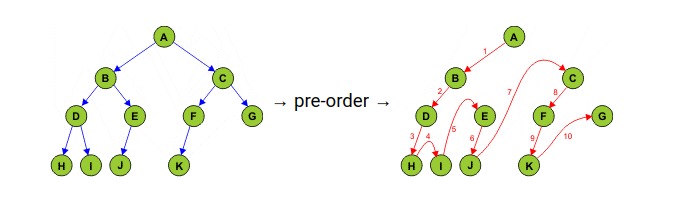
\includegraphics[width=0.4\textwidth]{../assets/5_3.png}} & PreOrder: A B D H I E J C F K G \\
\hline
\href{https://i.imgur.com/ZXdwmZn.png}{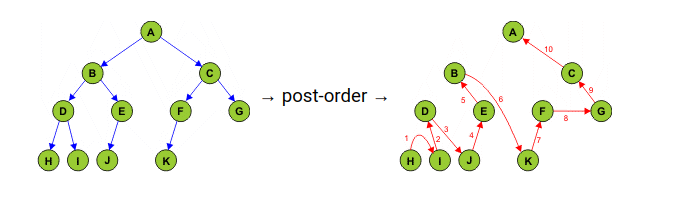
\includegraphics[width=0.4\textwidth]{../assets/5_1.png}} & PostOrder: H I D J E B K F G C A \\
\hline
\href{https://i.imgur.com/zMCdQRN.png}{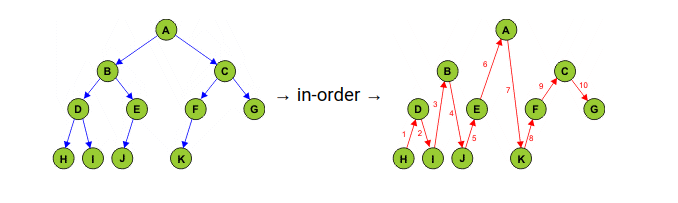
\includegraphics[width=0.4\textwidth]{../assets/5_2.png}} & InOrder: H D I B J E A K F C G \\
\hline
\end{tabular}
\end{table}

\section*{Wizualizacja operacjii}

\subsection*{Dodawanie}


\begin{tabular}{|>{\centering\arraybackslash}m{0.3\textwidth}|>{\centering\arraybackslash}m{0.7\textwidth}|}
    \hline
    \textbf{Stan} & \textbf{Opis} \\
    \hline
    \href{https://i.imgur.com/tZArpvb.png}{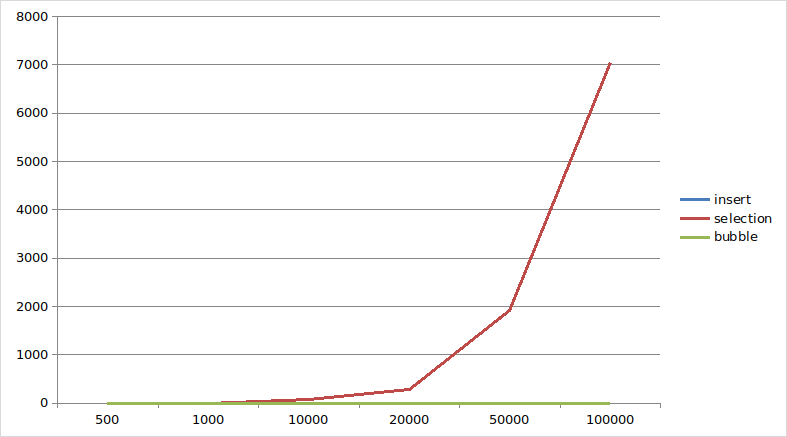
\includegraphics[width=0.2\textwidth]{"../assets/3_1.png"}} & Dodanie elementu o kluczu 4 jako korzenia drzewa.   \\
    \hline
    \href{https://i.imgur.com/tZArpvb.png}{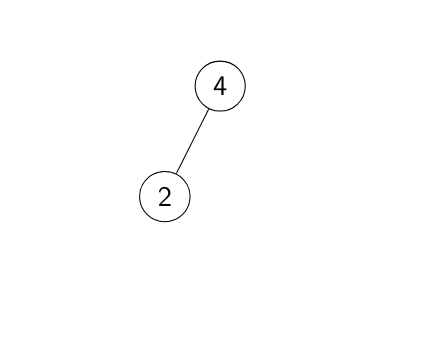
\includegraphics[width=0.2\textwidth]{"../assets/3_2.png"}} & Dodanie elementu o kluczu 2. Ponieważ 2 jest mniejsze niż 4, element zostaje umieszczony w lewym poddrzewie korzenia.    \\
    \hline
    \href{https://i.imgur.com/48XNmMa.png}{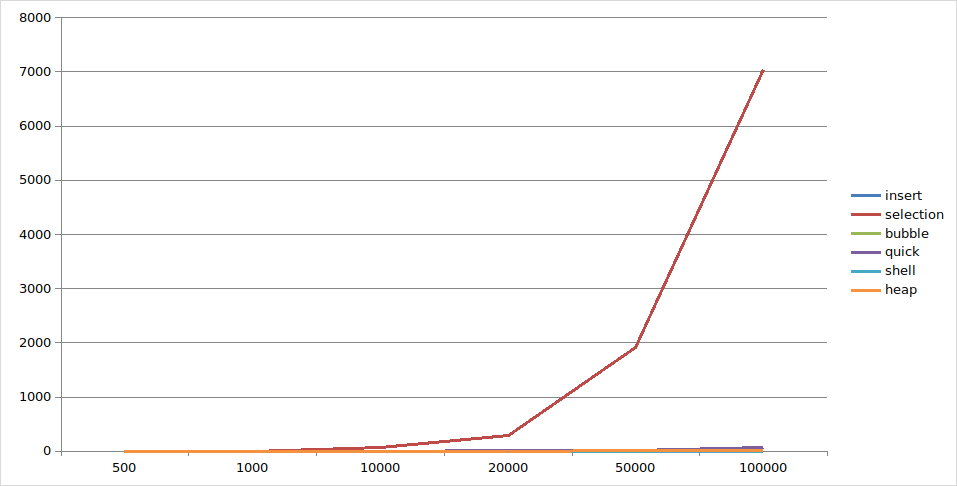
\includegraphics[width=0.2\textwidth]{"../assets/3_3.png"}} & Dodanie elementu o kluczu 1. Ponieważ 1 jest mniejsze niż 4 oraz mniejsze niż 2, element zostaje umieszczony w lewym poddrzewie węzła 2. \\
    \hline
    \href{https://i.imgur.com/c4sM6BP.png}{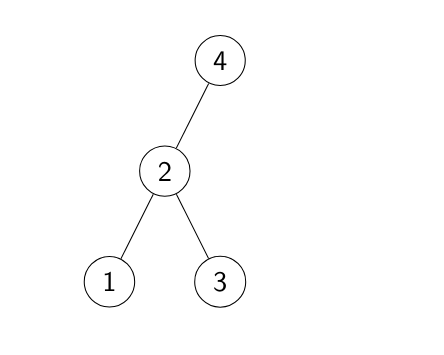
\includegraphics[width=0.2\textwidth]{"../assets/3_4.png"}} & Dodanie elementu o kluczu 3. Ponieważ 3 jest mniejsze niż 4, ale większe lub równe 2, element zostaje umieszczony w lewym poddrzewie korzenia i w prawym poddrzewie węzła 2. \\
    \hline
    \href{https://i.imgur.com/aRC3aUB.png}{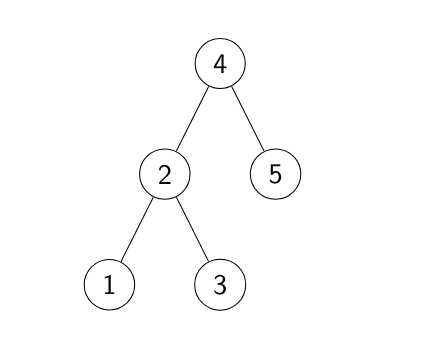
\includegraphics[width=0.2\textwidth]{"../assets/3_5.png"}} & Dodanie elementu o kluczu 5. Ponieważ 5 jest większe lub równe 4, element zostaje umieszczony w prawym poddrzewie korzenia. \\
    \hline
    \end{tabular}

\subsection*{Usuwanie}
Węzły usuwamy z drzewa BST, tak aby została zachowana hierarchia powiązań węzłów. Musimy rozpatrzyć kilka przypadków.

\begin{tabular}{|>{\centering\arraybackslash}m{0.3\textwidth}|>{\centering\arraybackslash}m{0.7\textwidth}|}
    \hline
    \textbf{Stan} & \textbf{Opis} \\
    \hline
    \href{https://i.imgur.com/MiukhDU.png}{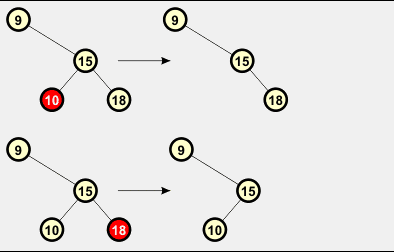
\includegraphics[width=0.2\textwidth]{"../assets/2_1.png"}} & Usuwany węzeł jest liściem, tzn. nie posiada synów. W takim przypadku po prostu odłączamy go od drzewa i usuwamy.    \\
    \hline
    \href{https://i.imgur.com/n1rgQ3G.png}{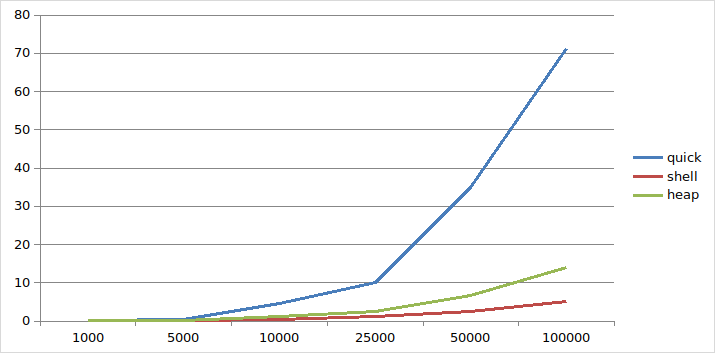
\includegraphics[width=0.2\textwidth]{"../assets/2_2.png"}} & Usuwany węzeł posiada tylko jednego syna. Węzeł zastępujemy jego synem, po czym węzeł usuwamy z pamięci.    \\
    \hline
    \href{https://i.imgur.com/IxPk8qc.png}{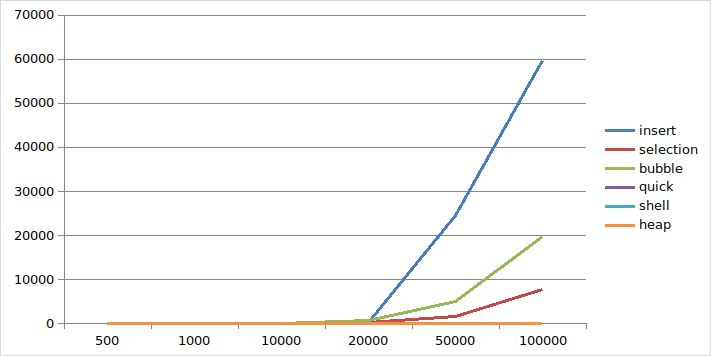
\includegraphics[width=0.2\textwidth]{"../assets/2_3.png"}} & Najbardziej skomplikowany jest przypadek trzeci, gdy usuwany węzeł posiada dwóch synów. W takim przypadku znajdujemy węzeł będący następnikiem usuwanego węzła. Przenosimy dane i klucz z następnika do usuwanego węzła, po czym następnik usuwamy z drzewa – do tej operacji można rekurencyjnie wykorzystać tę samą procedurę lub zastąpić następnik przez jego prawego syna (następnik nigdy nie posiada lewego syna). Jako wariant można również zastępować usuwany węzeł jego poprzednikiem. \\
    \hline
    \end{tabular}

\subsection*{Przeszukiwanie}
Drzewa BST pozwalają wyszukiwać zawarte w nich elementy z klasą złożoności obliczeniowej O (log n), gdzie n oznacza liczbę węzłów. Prześledźmy sposób wyszukiwania węzła o kluczu 19 w drzewie BST:

\begin{tabular}{|>{\centering\arraybackslash}m{0.3\textwidth}|>{\centering\arraybackslash}m{0.7\textwidth}|}
\hline
\textbf{Stan} & \textbf{Opis} \\
\hline
\href{https://i.imgur.com/JAxl8x6.png}{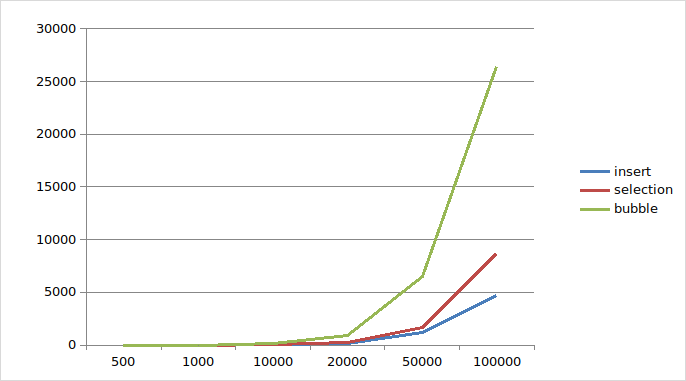
\includegraphics[width=0.2\textwidth]{"../assets/1_1.png"}} & Wyszukiwanie rozpoczynamy od korzenia drzewa. Porównujemy wartość węzła z wartością poszukiwaną. Ponieważ jest ona większa od wartości korzenia, idziemy wzdłuż prawej krawędzi do prawego syna (jeśli węzeł nie miałby prawego syna, to oznaczałoby to, że poszukiwanej wartości nie ma w drzewie BST). \\
\hline
\href{https://i.imgur.com/rmndQqe.png}{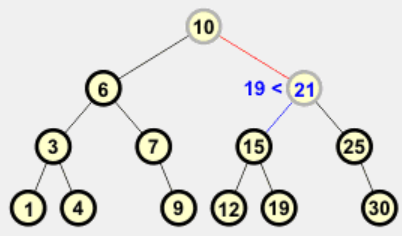
\includegraphics[width=0.2\textwidth]{"../assets/1_2.png"}} & W węźle 21 ponownie dokonujemy porównania. Ponieważ poszukiwany węzeł jest mniejszy od 21, wybieramy gałąź lewą i przechodzimy do lewego syna 15. \\
\hline
\href{https://i.imgur.com/XnmcQai.png}{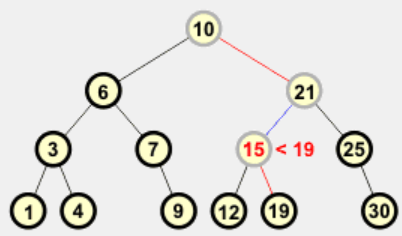
\includegraphics[width=0.2\textwidth]{"../assets/1_3.png"}} & Porównujemy węzeł 15 z poszukiwanym 19. Ponieważ 19 jest większe, idziemy prawą krawędzią do prawego syna 19. \\
\hline
\href{https://i.imgur.com/ngdZBi0.png}{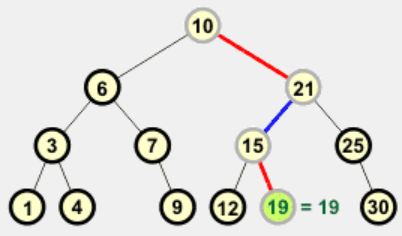
\includegraphics[width=0.2\textwidth]{"../assets/1_4.png"}} & Porównujemy węzeł 19 z poszukiwanym. Są równe. Wyszukiwanie zakończone. \\
\hline
\end{tabular}



\section*{Zlozonosc operacjii}

Podane testy zostały wygenerowane dla losowo wybranych danych z przedziału [0, SIZE]. Czasy przedstawione na wykresach są wyrażone w milisekundach.

\subsection*{Dodawanie N elemtnow}
\begin{figure}[H]
    \centering
    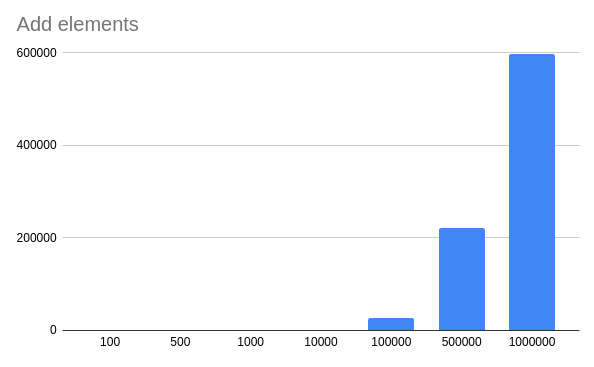
\includegraphics[width=\textwidth]{"../assets/4_1.png"}
    \label{fig:4_1}
\end{figure}

\subsection*{Dodawanie N + 1 elementu}

\begin{figure}[H]
    \centering
    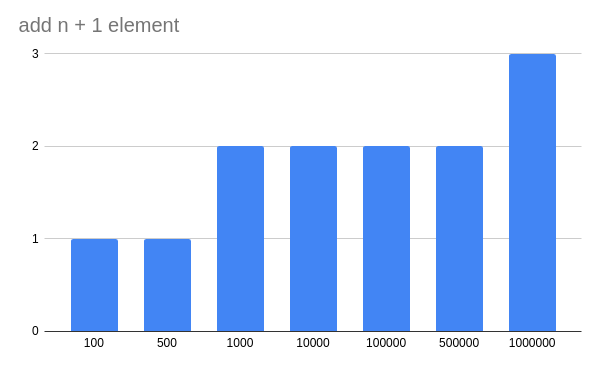
\includegraphics[width=\textwidth]{"../assets/4_2.png"}
    \label{fig:4_2}
\end{figure}


\subsection*{Usuwanie}

\begin{figure}[H]
    \centering
    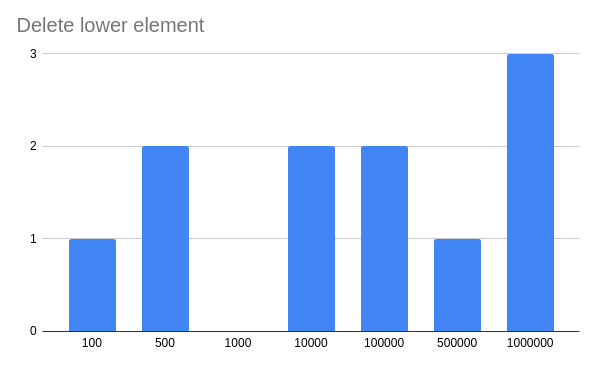
\includegraphics[width=\textwidth]{"../assets/4_6.png"}
    \caption{"Lower" oznacza element znajdujący się w dolnych 10 procent wysokości drzewa.}
    \label{fig:4_6}
\end{figure}

\begin{figure}[H]
    \centering
    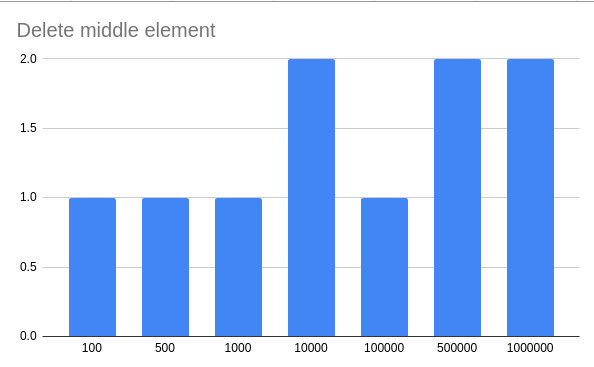
\includegraphics[width=\textwidth]{"../assets/4_7.png"}
    \caption{"Middle" oznacza element znajdujący się w zakresie od 10 procent do 40 procent wysokości drzewa. }
    \label{fig:4_7}
\end{figure}

\begin{figure}[H]
    \centering
    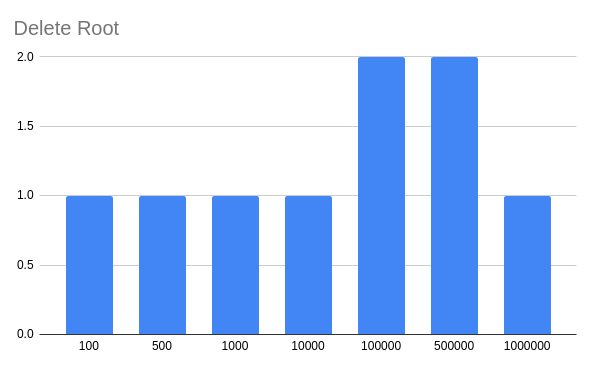
\includegraphics[width=\textwidth]{"../assets/4_8.png"}
    \label{fig:4_8}
\end{figure}



\subsection*{Przeszukiwanie}

\begin{figure}[H]
    \centering
    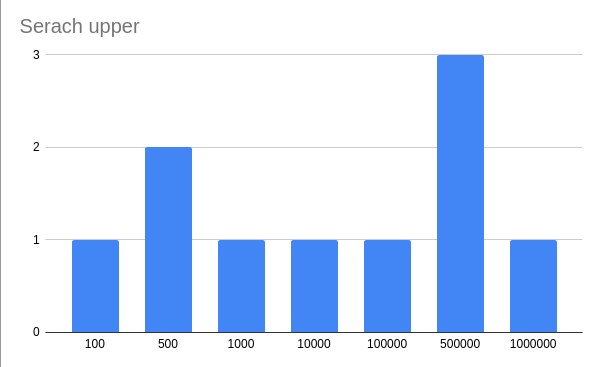
\includegraphics[width=\textwidth]{"../assets/4_3.png"}
    \caption{"Upper" oznacza element znajdujący się w zakresie od 40 procent do 100 procent wysokości drzewa.}
    \label{fig:4_3}
\end{figure}

\begin{figure}[H]
    \centering
    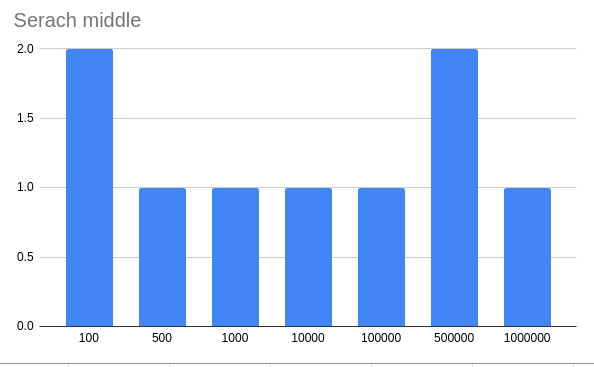
\includegraphics[width=\textwidth]{"../assets/4_4.png"}
    \caption{"Middle" oznacza element znajdujący się w zakresie od 10 procent do 40 procent wysokości drzewa. }
    \label{fig:4_4}
\end{figure}

\begin{figure}[H]
    \centering
    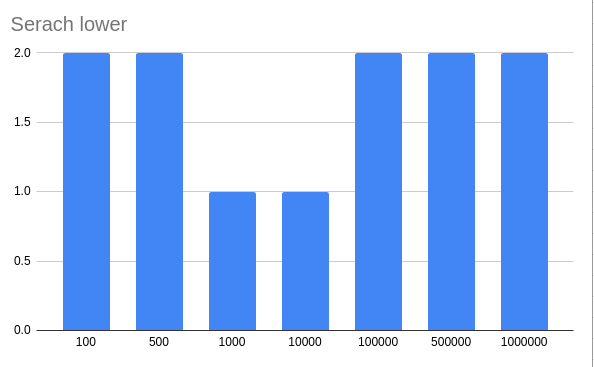
\includegraphics[width=\textwidth]{"../assets/4_5.png"}
    \caption{"Lower" oznacza element znajdujący się w dolnych 10 procent wysokości drzewa.}
    \label{fig:4_5}

\end{figure}

\subsection*{Wykres zbiorczy}

\begin{figure}[H]
    \centering
    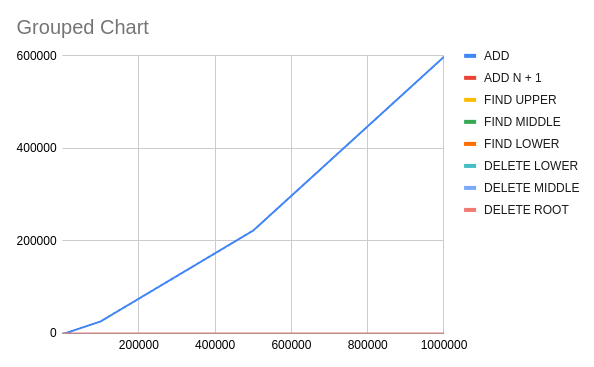
\includegraphics[width=\textwidth]{"../assets/4_9.png"}    
    \label{fig:4_9}

\end{figure}

\subsection*{Wyniki przeprowadzonych testów}

\begin{table}[H]
    \begin{tabular}{|l|r|r|r|r|r|r|r|}
    \hline
    {[}ms{]}      & 100 & 500 & 1000 & 10000 & 100000 & 500000 & 1000000 \\ \hline
    ADD           & 7   & 44  & 91   & 1284  & 26117  & 222522 & 598058  \\ \hline
    ADD N + 1     & 1   & 1   & 2    & 2     & 2      & 2      & 3       \\ \hline
    FIND UPPER    & 1   & 2   & 1    & 1     & 1      & 3      & 1       \\ \hline
    FIND MIDDLE   & 2   & 1   & 1    & 1     & 1      & 2      & 1       \\ \hline
    FIND LOWER    & 2   & 2   & 1    & 1     & 2      & 2      & 2       \\ \hline
    DELETE LOWER  & 1   & 2   & 0    & 2     & 2      & 1      & 3       \\ \hline
    DELETE MIDDLE & 1   & 1   & 1    & 2     & 1      & 2      & 2       \\ \hline
    DELETE ROOT   & 1   & 1   & 1    & 1     & 2      & 2      & 1       \\ \hline
    \end{tabular}
    \end{table}

\section*{Podsumowanie}
Na podstawie przeprowadzonych testów oraz ich wyników widzimy wydajność drzewa BST po przeprowadzeniu konkretnych operacji względem tego ile jest zawartych w nim elementów, Wyniki testów wydajnościowych potwierdzają, że drzewo BST jest skuteczną strukturą danych do przechowywania i manipulowania zbiorem danych. Czas operacji dodawania wielu elementów gwałtownie wzrasta, w zależości od ich liczby. W przypadku dodawania, wyszukiwania czy też usuwania pojedyńczego elementu czas ten nie przekracza 3[ms] co pokazuje jak bardzo drzewo BST jest efektywne w tego typu zabiegach. 



\end{document}